
\section*{Weighted mean}

The weighted mean is the same as the mean, except that it is influenced more by some observations than others. We assign weights to observations as a sort of way of describing its relative importance. In many applications, there are natural choices for weights. For example, in the \data{county} data set, population is a natural weighting factor.

Given the number of people in each county of the United States and also the average income per person in each county, how should we compute the average income per person for residents in the United States?

An initial guess might ignore the population data. This would yield a mean income of about \$22,505. However, this is not the mean income of the people in the United States, which is actually several thousand dollars more. To see why, consider Figure~\ref{incomeVsPop}, which shows the income and population of all 3,143 counties. Notice first that the scale on the horizontal axis for population shows a special scale (called the log-scale). Many of the biggest counties have higher incomes than the smaller counties. This is why our original mean calculation gives a wrong answer.
\begin{figure}
\centering
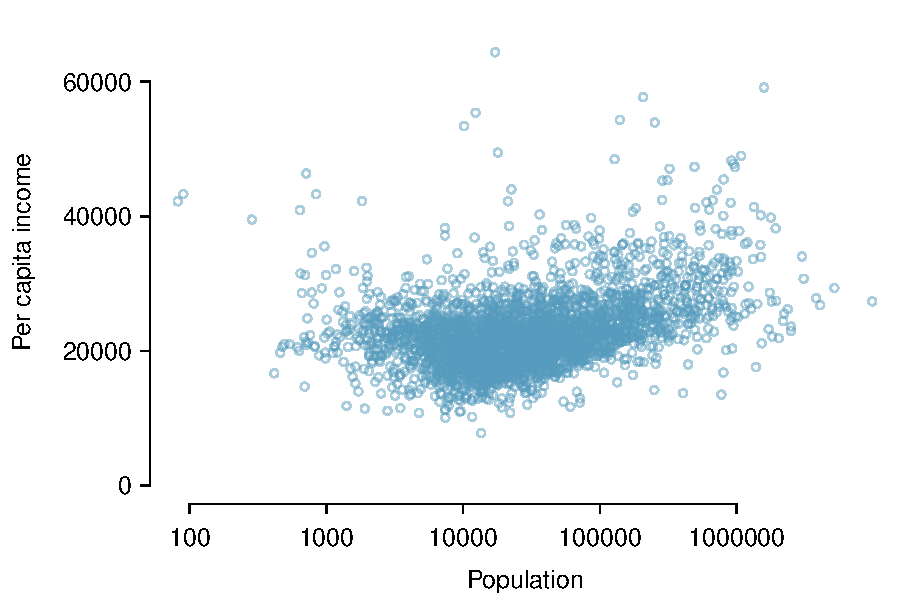
\includegraphics[width=\textwidth]{WeightedMean/figures/incomeVsPop/incomeVsPop} 
\caption{Per capita income against population size in 3,143 US counties.}
\label{incomeVsPop}
\end{figure}

Let's think again about the regular problem: we want the mean income per person in the United States. We need exactly two numbers to complete this calculation: the total income of all people in the US and the number of people in the US:
\begin{align*}
\frac{\text{Total income of all people in the US}}{\text{Number of people in the US}}
\end{align*}
We're not given these numbers, but the data provided is sufficient to calculate each of the numbers. Starting with the denominator (the bottom), just add up the population in all the counties: 308,745,538.

The numerator (the top of the fraction) is a little tougher, but not much. If we had the total income of all people each county, then we could add up all those values to get the total income. To get the income for any given county, we can multiple the average income of the county with the number of people in the county. This just relies on a rearrangement of the equation defining the average income for the county:
\begin{align*}
\text{Ave income} = \frac{\text{County income}}{\text{Num. people in county}}
\end{align*}
\begin{align*}
\Downarrow
\end{align*}
\begin{align*}
(\text{Ave income})(\text{Num. people in county}) = \text{County income}
\end{align*}
Now that we can get the county incomes, we can get the income for the entire United States: about \$8.4447 trillion (\$8,444,700 million). Finally, we can calculate the average income in the United States:
\begin{align*}
\frac{\text{Total income of all people in the US}}{\text{Number of people in the US}}
	= \frac{\text{\$8,444,700,000,000}}{\text{308,745,538}} = \$27,348
\end{align*}
Recall that the simple mean was \$22,505.

Let's put the entire calculation into a single expression. We'll use $w_1$ to represent the population of the first county, $w_2$ to represent the population of the second county, and so on. The label $x_1$ will represent the average income of county 1, $x_2$ for the average income of county 2, and so on. Then the mean weighted by population can be written as
\begin{align*}
\frac{w_{1}x_{1} + w_{2}x_{2} + w_{3}x_{3} + \dots + w_{3143}x_{3143}}
	{w_{1} + w_{2} + w_{3} + \dots + w_{3143}}
\end{align*}
This equation represents the \term{weighted mean} of income, where the weights are given by the population values.

\begin{termBox}{\tBoxTitle{Weighted mean}
The weighed mean of observations $x_1$, $x_2$, ..., $x_n$ using weights $w_1$, $w_2$, ..., $w_n$ is given by
\begin{align*}
\text{weighted mean of $x_i$s} = 
\frac{w_{1}x_{1} + w_{2}x_{2} + \dots + w_{n}x_{n}}
	{w_{1} + w_{2} + \dots + w_{n}} = 
\frac{\sum_{i=1}^n w_{i}x_{i}}
	{\sum_{i=1}^n w_{i}}
\end{align*}
If the second equation with the $\Sigma$s isn't math notation you feel comfortable with, just consider the first definition. The second expression is just a fancy way of making the equation compact.}\end{termBox}

\begin{tipBox}{\tipBoxTitle{Simple mean is a special case of the weighted mean}
The simple mean is a weighted mean where all the weights are~1:
\begin{align*}
\frac{x_{1} + x_{2} + x_{3} + \dots + x_{n}}
	{n}
= \frac{1\times x_{1} + 1\times x_{2} + 1\times x_{3} + \dots + 1\times x_{n}}
	{1 + 1 + 1 + \dots + 1}
\end{align*}
}\end{tipBox}
The ideas of weighted means are important to some methods that are usually encountered in a second or later course in statistics. We don't touch on the topic again in \emph{OpenIntro Statistics}.

%===============
%\pagebreak
%
%The exercises below are not based on real data.
%
%\begin{exercise}
%Stratified sampling is useful when selecting a specific fraction of observations from groups in a population. Suppose we are given groups of the following sizes from each of these populations:
%\begin{center}
%\begin{tabular}{l cc l cc}
%    & \multicolumn{2}{c}{Population} && \multicolumn{2}{c}{Sample} \\
%\cline{2-3} \cline{5-6}
%    & Size & Fraction && Size & Mean Satisfaction \\
%\hline
%Agriculture and Veterinary	& 486	&	&& 30 	& 5.9 \\
%Arts and Design			& 1,192	& 	&& 30 	& 7.2 \\
%Engineering				& 2,410	& 	&& 40 	& 7.7 \\
%Hard Sciences and Math		& 2,882	& 	&& 40 	& 6.8 \\
%Health and Medical			& 1,581	& 	&& 40	& 6.3 \\
%Languages				& 1,257	& 	&& 30	& 5.2 \\
%Social Sciences			& 3,925	& 	&& 50 	& 6.5 \\
%\hline
%\end{tabular}
%\end{center}
%First, notice that while the sample sizes are larger for larger groups, they are not proportionally larger. If the only goal of the sample was to estimate the total population mean, we might have picked proportional sample sizes. However, the sample sizes of all groups was at least 30 to provide a somewhat stable estimate for each group of majors, which is represented in the last column.
%
%The overall population mean can be estimated using the group means. However, like with the income per capita, these mean satisfaction values provided each represent different sized subpopulations. For this reason, a weighted mean is necessary. Calculate the weighted mean of satisfaction where the weights are the population fraction.
%\end{exercise}

































